%
% File: thesisexample.tex   Version 1.8   May 6, 1999
%
% This is an example document for easychithesis, a 
% LaTeX2e style for formating theses at the University of
% Chicago.The easychithesis style was written by Bryan Clair and 
% Nathan Dunfield.  It contains detailed instructions for using
% easychithesis.
%
%  HINTS:
%
%  1. To get appendices, you don't do anything different from a normal
%     report document.  That means, put the command \appendix before
%     you begin your first appendix, then do each appendix with a
%     \chapter command.  Note that if you have only one appendix, it is
%     customary to leave it unnumbered.  Do this with \chapter*.
%
%  2.  If you use \chapter*, which produces unnumbered chapters, you 
%       have to add that chapter to the table of contents by hand, e.g.
%
%         \chapter*{Appendix}
%         \addcontentsline{toc}{chapter}{Appendix}
%
%  3.  If you get errors about
%   
%    Undefined control sequence.
%         \setspace@size ...rrsize \normalsize \@normalsize \else \@currsize \fi 
%
%     You need a newer version of the file ``setspace.sty''.
%
%  4.  Problems with math formulas in chapter headings:
% 
%         a.  Any lowercase letters in the formula are converted to
%         uppercase, e.g. f(x) becomes F(X).   If you really need
%         lowercase math letters in your chapter titles, use the
%         option plainchapterheads (and, if you want, type your
%         chapter titles in ALL CAPS so that the appearance doesn't
%         change).  Note there is no problem 
%         for section or subsection headings in either case.  (Options
%         such as plainchapterheads are given as part of the 
%         \documentclass command, see below under ``Document Options'').
%
%         b.  Some perfectly reasonable math commands when used in
%         \chapter give the error
%          ``LATEX ERROR: \command  ALLOWED ONLY IN MATH MODE.''
%         The solution to this is to do
%        
%              \newcommand{\mymath}{problem math goes here}
%       
%         and then
%        
%              \chapter{All about \protect\mymath}
%
%         also, the option plainchapterheads will fix this too.
%
%  5. If your References section doesn't show up in the table of
%     contents, you need to add the line \addcontentsline...
%     as done at end of this file.   Make sure that you include the 
%     page break command as done there or else you may end up
%     with the wrong page number in your table of contents. 


\documentclass{easychithesis}
% \bibstyle{plos2009}

%PLOS Packages
% amsmath package, useful for mathematical formulas
\usepackage{amsmath}
% amssymb package, useful for mathematical symbols
\usepackage{amssymb}

% graphicx package, useful for including eps and pdf graphics
% include graphics with the command \includegraphics
\usepackage{graphicx}
\usepackage{subfigure}

% cite package, to clean up citations in the main text. Do not remove.
\usepackage{cite}
\usepackage{color}

% Use doublespacing - comment out for single spacing
%\usepackage{setspace} 
%\doublespacing

% Document Options: 
%
% Note if you want to save paper when printing drafts, replace the
% above line by
% 
%   \documentclass[singlespace]{easychithesis}
% 
% or 
% 
%   \documentclass[onehalfspace]{easychithesis}
%
% Also the ``double spacing'' provided by this style is not ``true''
% doublespacing as defined by setspace.sty.  Instead, it is the same
% as on the old LaTeX 2.09 thesis style ``chithesis''.  If you want 
% ``true'' doublespacing (if there is such a thing), give the option 
% truedoublespace.  The increase in tree murder will be on your 
% conscience, not mine.
%
%  Similarly, if you need to use the plainchapterheads option, you do
%   
%  \documentclass[plainchapterheads]{easychithesis}
%
% You can give more than one option, if you desire.

\begin{document}

% Create the official title
\title{Detecting SVs in Cancer Genomes Through Direct Cancer/Somatic Comparison} 
\author{Cody Weinberger}
\date{December 2014}
\department{Ecology and Evolution}
\division{Biological Sciences} 
\degree{Bachelor of Science with Honors in Biology} 
\maketitle

% \dedication : Use for a dedication, copyright, or epigraph.
%               Produces a page with no number for the text which follows
%               If you want centering, do it yourself with 
%               \begin{center} and \end{center}.  You can have more
%               than one `dedication'.
%\dedication
%\begin{center}
%        To Someone TBD
%\end{center}


% \topmatter : Things like Abstract, Acknowledgements.
% For the abstract, you can also do 
%      \begin{abstract} ...text... \end{abstract}
% if you prefer.

\topmatter{Abstract}
As next generation sequencing technology (NGS) increasingly allows for cheap sequencing of entire genomes, the challenge of obtaining accurate sequences is largely computational. While it has become routine to detect single nucleotide polymorphisms, detecting large scale structural variants (SVs) is a much more complex issue primarily due to short read length. A promising avenue of SV detection is using soft-clipped reads, which allows for single nucleotide resolution of potential breakpoints. When using NGS to detect somatic mutations, the traditional approach has been to compare both somatic and cancer soft-clipped reads to a reference and subtract the somatic breakpoints from the cancer breakpoints to obtain those that have occurred only in somatic cells. However, comparing the cancer and somatic genomes indirectly prevents detection of some types of mutatons, e.g. any mutation nested within a novel inserton. There is also a large bias towards detecting deletons over insertions using this method, as novel regions of soft-clipped reads cannot map to the reference. A method for comparing cancer and somatic genomes directly is presented here to avoid these issues.

\topmatter{Acknowledgements}
I'd like to thank Wen-Hsiung Li for agreeing to advise and host me and my project at Academia Sinica. I'd also like to thank Stefano Allesina for providing me with research experience and advising this project. Thank you to Jason Tsai for comments and discussion. This research was supported by UChicago SITG and Academia Sinica TIGP-IIP.

%
% Table Of Contents
%

\tableofcontents

%
% List of figures
% 

\listoffigures

% 
% List of tables
% 

\listoftables

%
% Begin Body
%
\mainmatter

%
% Body Chapters
%
\chapter{Introduction}
\section{Next-Generation Sequencing}
[A review of the advances and utility of next-gen sequencing.] Recent developments in sequencing technology now can generate reads up to ~300bp with large genomic coverage for a low cost. Further, exome sequencing can be done with minimal time and cost. This is opening a new avenue of medicine - personal genomics - to become a real, affordable option to diagnose uncommon diseases \cite{pabinger2014survey, feuk2006structural}. By investigating which genes are being affected in an individual, we can actually target the cause of the disease, e.g. which protein is being altered or suppressed. Ease of sequencing also allows us to sequence both healthy somatic cells and cancer tumor cells in a given individual, opening another avenue of more detailed cancer diagnosis and case-specific treatment.

\section{Detecting Structural Variants}
[A review of the general approaches to detecting SVs.] There are now a few different approaches to detecting potential breakpoints between structural variants. Each has its own advantages and pitfalls, and generally multiple approaches are used in combination to improve confidence and the discovery rate of breakpoints.

\subsection{Discordant Pair Approach}
Many sequencing methods utilize paired-end sequencing, where each end of a read is sequenced, and thus we have two sequences with a known insert size, or distance apart from one another. This information can be utilized to detect SVs by checking if each paired end maps to the reference a distance equal to the insert size apart from one another. If the mapped distance is greater than expected, for example, then we suspect there has been an insertion event. If, conversely, the mapped distance is less than the insert, then we would call a deletion event. If only one sequence maps to the reverse of a match on the reference, then we suspect an inversion has occurred. This method is effective on small data sets and can be used with low depth of coverage and short reads \cite{suzuki2011clipcrop}. However, it cannot detect SVs that have short indels, as this will be indistinguishable from the approximate insert size \cite{abel2013detection, pabinger2014survey}. It also is not suited for detecting the exact positions of breakpoints, as the event is expected to have occured between the two paired ends, and does not output the actual inserted sequence \cite{abel2013detection}. Softwares that utilize this method include BreakDancer, VariationHunter, MoDIL, and ABI Tools \cite{suzuki2011clipcrop}.

\subsection{Depth of Coverage Approach}
We can utilize the differing levels of coverage between regions to detect insertions and deletions. If we have twice as many reads for a given region, for example, then we expect this region has been duplicated once. If it has three times as many reads, then it may have been duplicated twice. This method does not require paired-end data, but requires very high coverage to lower missed or overcovered regions due to chance. It also cannot tell you where the duplication has occured or whether it is tandem, especially if the region is large\cite{suzuki2011clipcrop}. Short SV events are not easily detected with this method. It is useful, however, in detecting copy number in large events, as other methods that rely solely on sequence have difficulty distinguishing between repetitive regions \cite{suzuki2011clipcrop}. Thus this method is often used in conjunction with more reliable methods to fill the void of detecting copy number SVs. Tools that utilize this method include SegSeq, CNVnator, and ABI Tools \cite{suzuki2011clipcrop}.

\subsection{Split-Read/Soft-Clipping Approach}
The split-read approach utilizes "unsuspected" reads, which do not fully map to the reference. Because an SV by definition causes the region flanking the breakpoint to differ than the reference on one side, any read spanning the boundary cannot contiguously map to the reference. If partially mapped or mapped to different regions, these reads are expected to span a breakpoint. Most methods utilize orphaned reads, which are unmapped but have a mate mapped to the reference. These are then used to flag potential SV boundaries, as a succesfully mapped mate reduces noise. The split-read method can detect SVs with single-base resolution, as the breakpoint is contained within a single read \cite{schroder2014socrates, suzuki2011clipcrop}. However, it requires high depth of coverage and longer read lengths\cite{suzuki2011clipcrop}. Tools that utilize this method include Pindel, PRISM, and SLOPE.

Another split-read method is the soft-clipped sequence approach. A soft-clipped read is only partially mapped to the reference. Thus again it likely spans over the boundary of an SV event. Tools that utilize this method include the Burrows-Wheeler alignment tool, ClipCrop, CREST, and Socrates. Because it allows for single breakpoint resolution, and should have the capability of detecting any type of SV event, this method is very promising. We use Socrates \cite{schroder2014socrates}, a recent and high-performing SV detection program, in our pipeline.

\section{Finding Somatic Mutations}
\subsection{Germline vs Somatic Mutations}
Mutations can occur either in somatic cells throughout the body, or in germline cells that are then passed onto the offspring. Germline mutations occur mainly in sperm due to the high number of cell divisions in sperm production. We are interested in somatic mutations, however, as we want to expose and treat the mutation that has allowed uninhibited cancer cell growth, which occurs almost exclusively after infancy and in somatic genomes.

\subsection{Traditional Approach and Shortcomings}
The traditional approach to finding somatic mutations compares both the somatic and cancer reads to the established reference genome and subtracts the differences \cite{schroder2014socrates, suzuki2011clipcrop, christoforides2013identification}. Any variation from the reference that occurs in the individual of interest, which is common due to high population-level variation between individuals, will be detected in the somatic genome, but also the cancer genome, as it is derived from the somatic. Because these individual variants are detected in both genomes, they are not counted as a somatic mutation.

By contrast, any change that has occurred between the somatic and cancer genomes will not be detected as a change from the reference to somatic, but will be from the reference to cancer genome. This is thus counted as a somatic mutation.

However, a problem arises when a somatic mutation has occured within the boundaries of a region not present in the reference. This may occur frequently due to high levels of population-level variation. Thus there are many regions of an individual's genome that are not represented in the human reference genome \cite{feuk2006structural}. The problem is that any indel that is contained in a novel region, e.g. not in the reference, cannot be detected through this indirect method. In the case of a novel region, only the boundaries of the novel region can be detected. Its flanking regions will be detected as breakpoints in the somatic genome. However, because the whole interior region is novel, no further novel indel breakpoints can be detected within the region. Thus any somatic indel's breakpoints cannot be distiniguished from an existing novel region, and only the region's outermost breakpoints will again be detected in the cancer genome. Then because only these widest breakpoints are detected both in the somatic and cancer genomes, they are subtracted and no somatic SV is called.

Another problem is that detection of deletions is biased over that of novel insertions, which has been noted as a problem with all existing methods \cite{lee2008robust, medvedev2009computational, jiang2012prism, abel2013detection, alkan2011genome}. Large insertions are especially elusive \cite{abel2013detection}, and some papers do not even consider the category of large insertions \cite{jiang2012prism}. Note that in the traditional method of comparing both the somatic reads to the reference and the cancer reads to the reference, we are only mapping the reads in one direction, e.g. from the sample to the reference. When a region is present in the reference, but not the sampled genome being mapped to the reference, the reads from the sampled genome will span the single breakpoint, and each side will map to the respective region flanking the "deleted" region in the reference. Thus 2 breakpoints on the reference and the single breakpoint on the sampled genome are detected. In the case of a novel insertion in the sampled genome relative to the reference, however, a read that spans either breakpoint in the sampled genome will be composed one part that maps to a flanking region in the reference, as in a deletion, but the other side will be a novel region that cannot map to the reference. Thus only half of the available power is available to call this breakpoint in the reference, and more of these events are missed. This bias is well illustrated in the call statistics of Socrates, where 94\% of deletions were called, but only 66\% of novel insertions \cite{schroder2014socrates}.

\begin{figure}[!ht]
\begin{center}
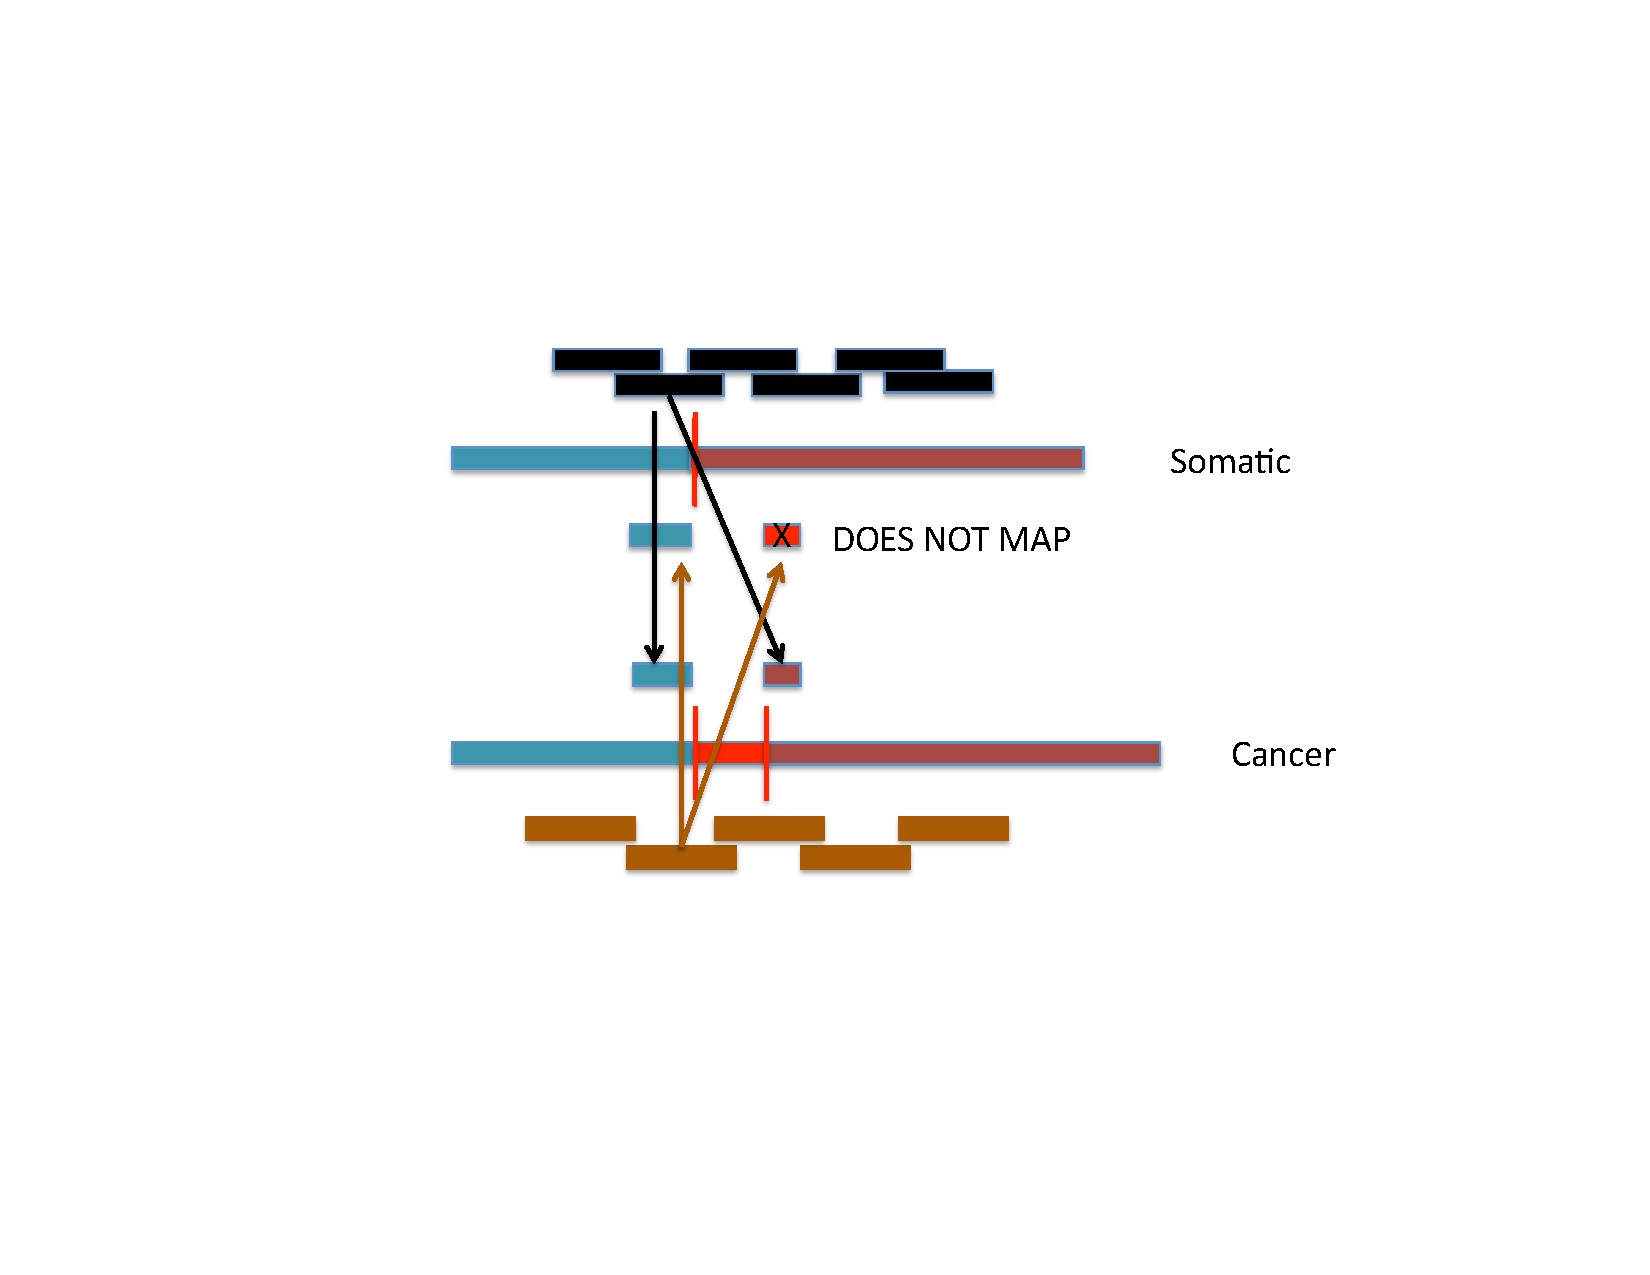
\includegraphics[width = 0.95  \linewidth]{../Code/Figures/DeletionBias.pdf}
\end{center}
\caption{{\bf Deletion bias of unidirectional mapping.} In the case of a novel insertion in the cancer genome, a cancer split-read will only have one part map to the somatic, as the novel region does not match anywhere on the genome. However, both parts of a somatic split-read will map to the cancer genome, each part flanking the novel insert. Having both parts of the split-read map to the opposing geneme greatly improves the SV discovery rate and confidence.}
\label{fig:DeletionBias}
\end{figure}

\subsection{Direct Somatic/Cancer Comparison}
The proposed method helps overcome the shortcomings of the traditional method primarily by comparing the two genomes directly. 

\begin{figure}[ht]
\centering
\subfigure[Indirect Comparison]{%
	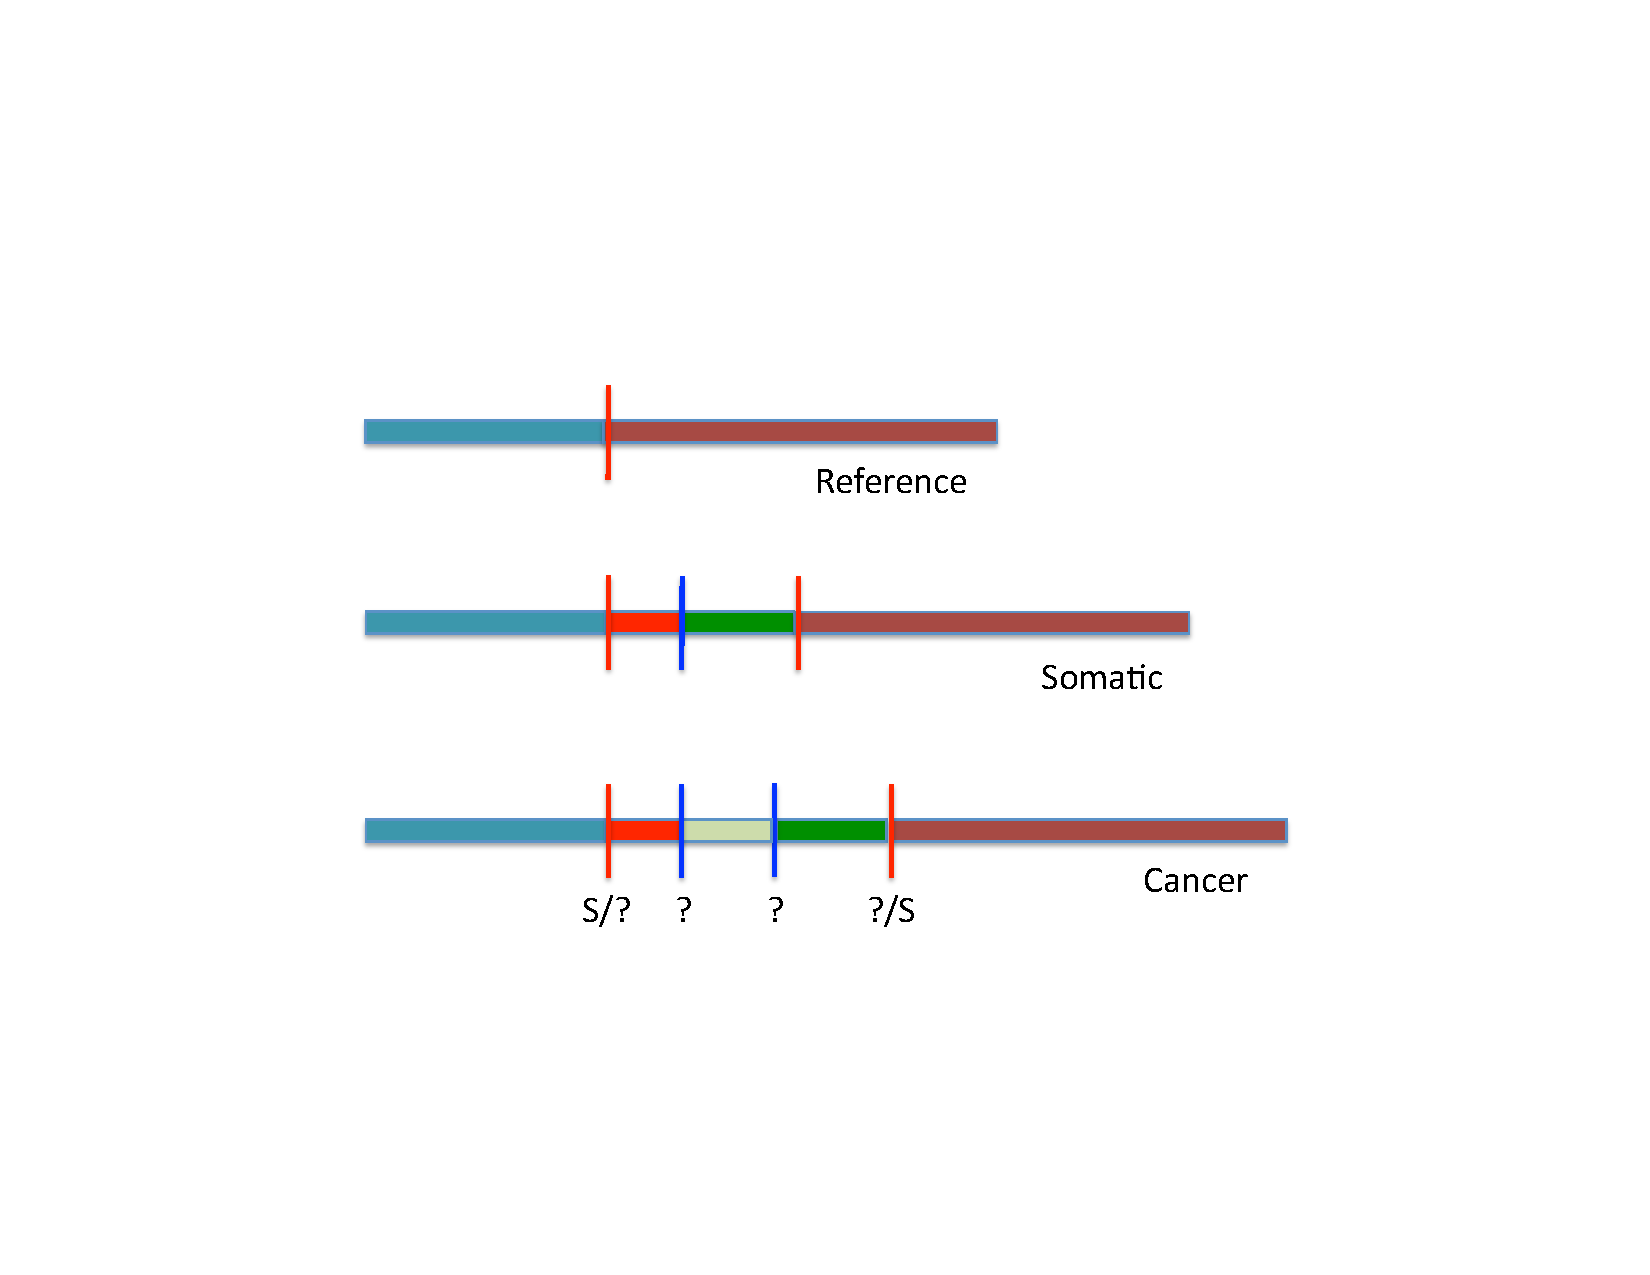
\includegraphics[width = 0.95  \linewidth]{../Code/Figures/InsertionIndirect.pdf}
	\label{fig:InsertionIndirect}}
\quad
\subfigure[Direct Comparison]{%
	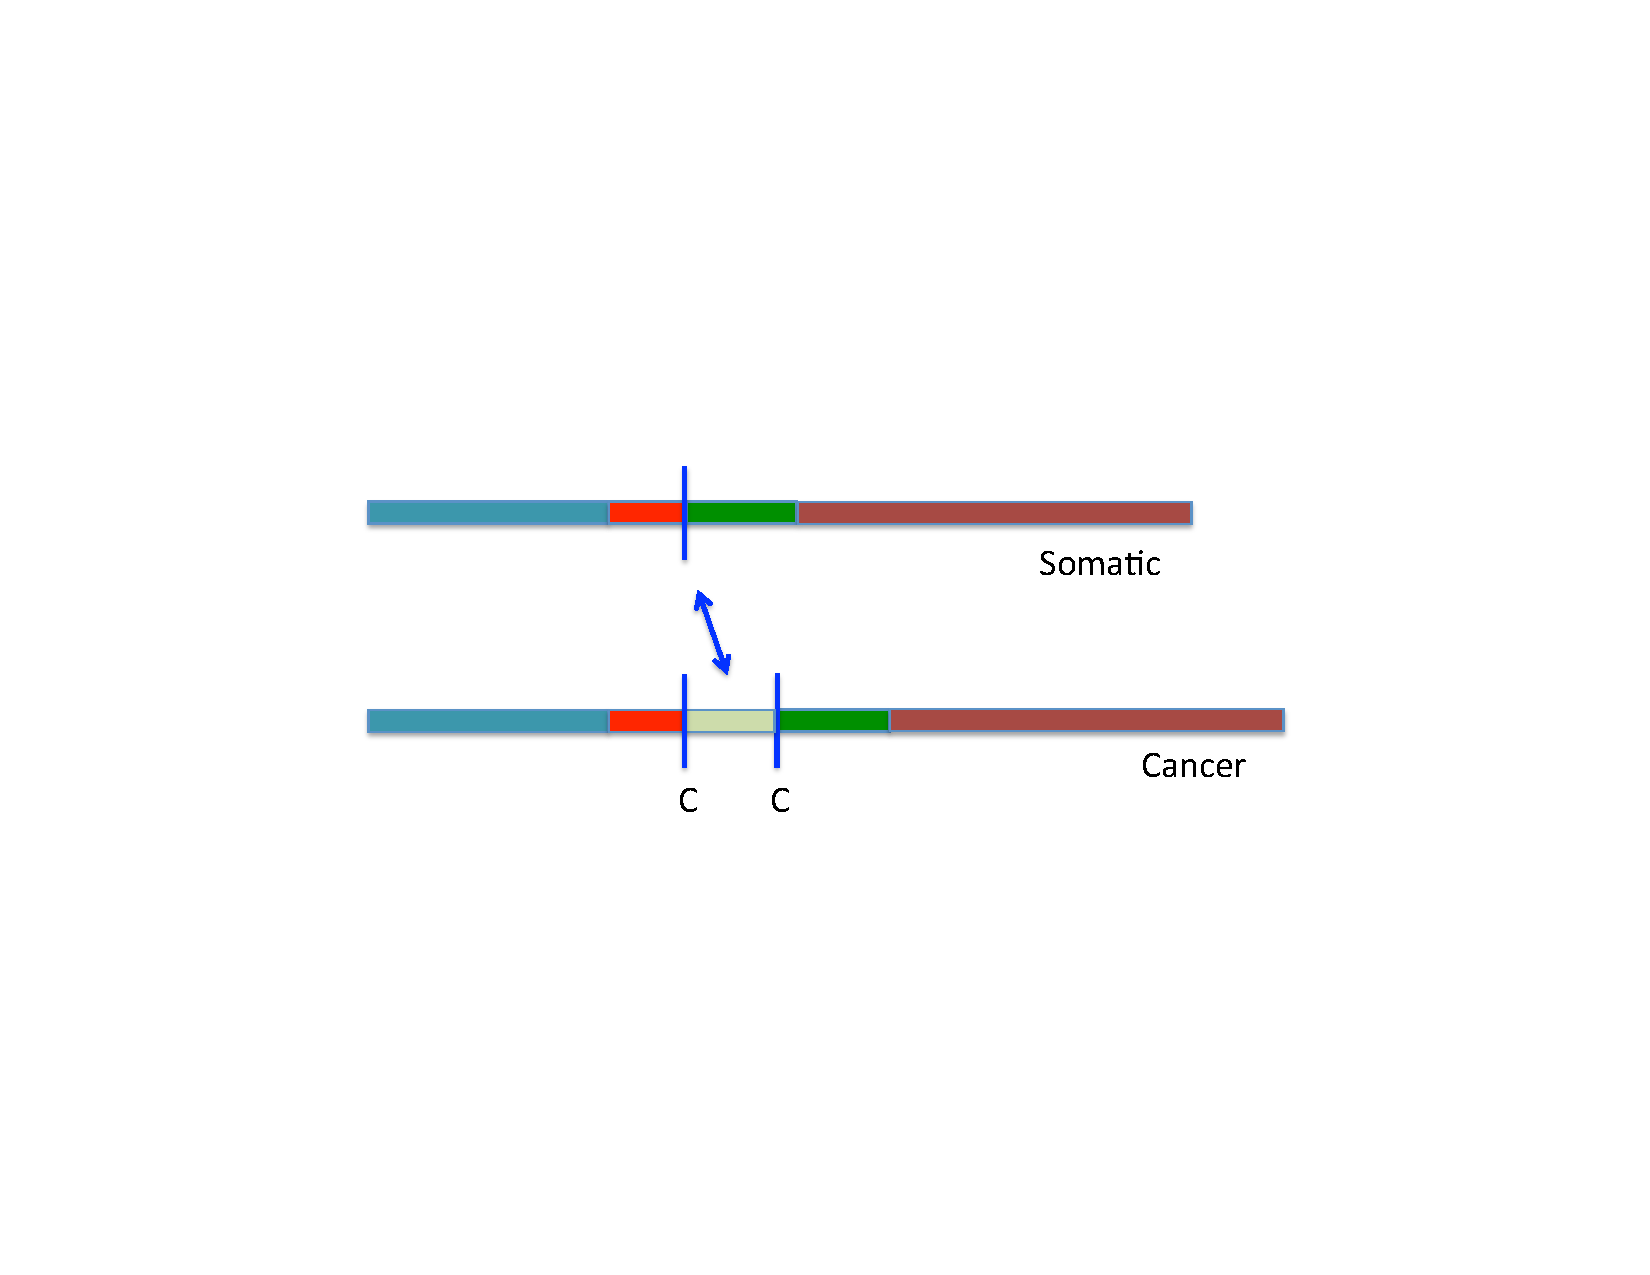
\includegraphics[width = 0.95  \linewidth]{../Code/Figures/InsertionDirect.pdf}
	\label{fig:InsertionDirect}}
%
\caption{{\bf Indirect vs direct comparison of nested insertion.} In the indirect comparison, the entire inner region, whether with or without an additional somatic insertion, is novel and thus only its outer breakpoints are detected. These outer breakpoints, however, are not somatic mutations and are present in both the somatic and tumor genomes. Thus the inner breakpoint is overlooked. The direct comparison, in contrast, ignores the outer breakpoints, as they are not different from the somatic to cancer genomes (only differ between genomes and reference). It instead only directs the somatic breakpoints, as these differ between the somatic and cancer genomes.}
\label{fig:NestedInsertion}
\end{figure}

\begin{figure}[ht]
\centering
\subfigure[Indirect Comparison]{%
	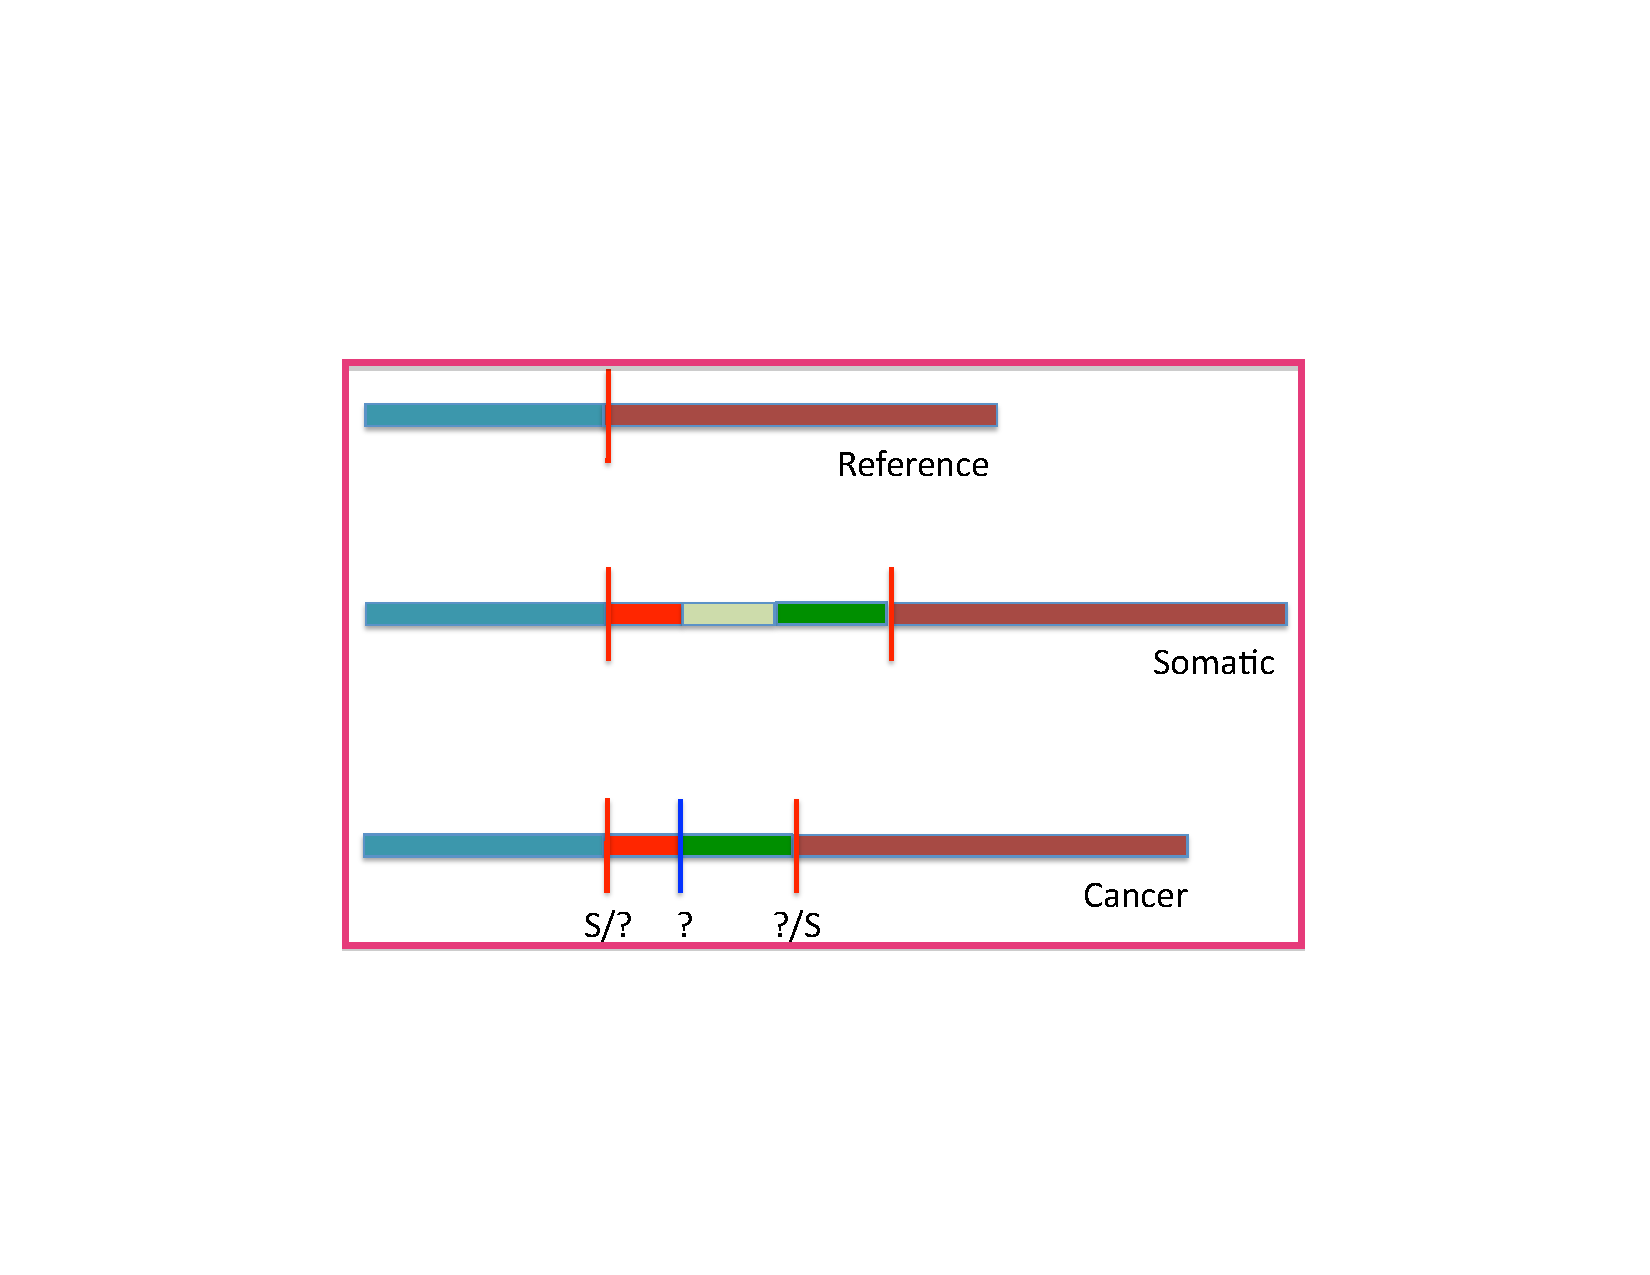
\includegraphics[width = 0.95  \linewidth]{../Code/Figures/DeletionIndirect.pdf}
	\label{fig:DeletionIndirect}}
\quad
\subfigure[Direct Comparison]{%
	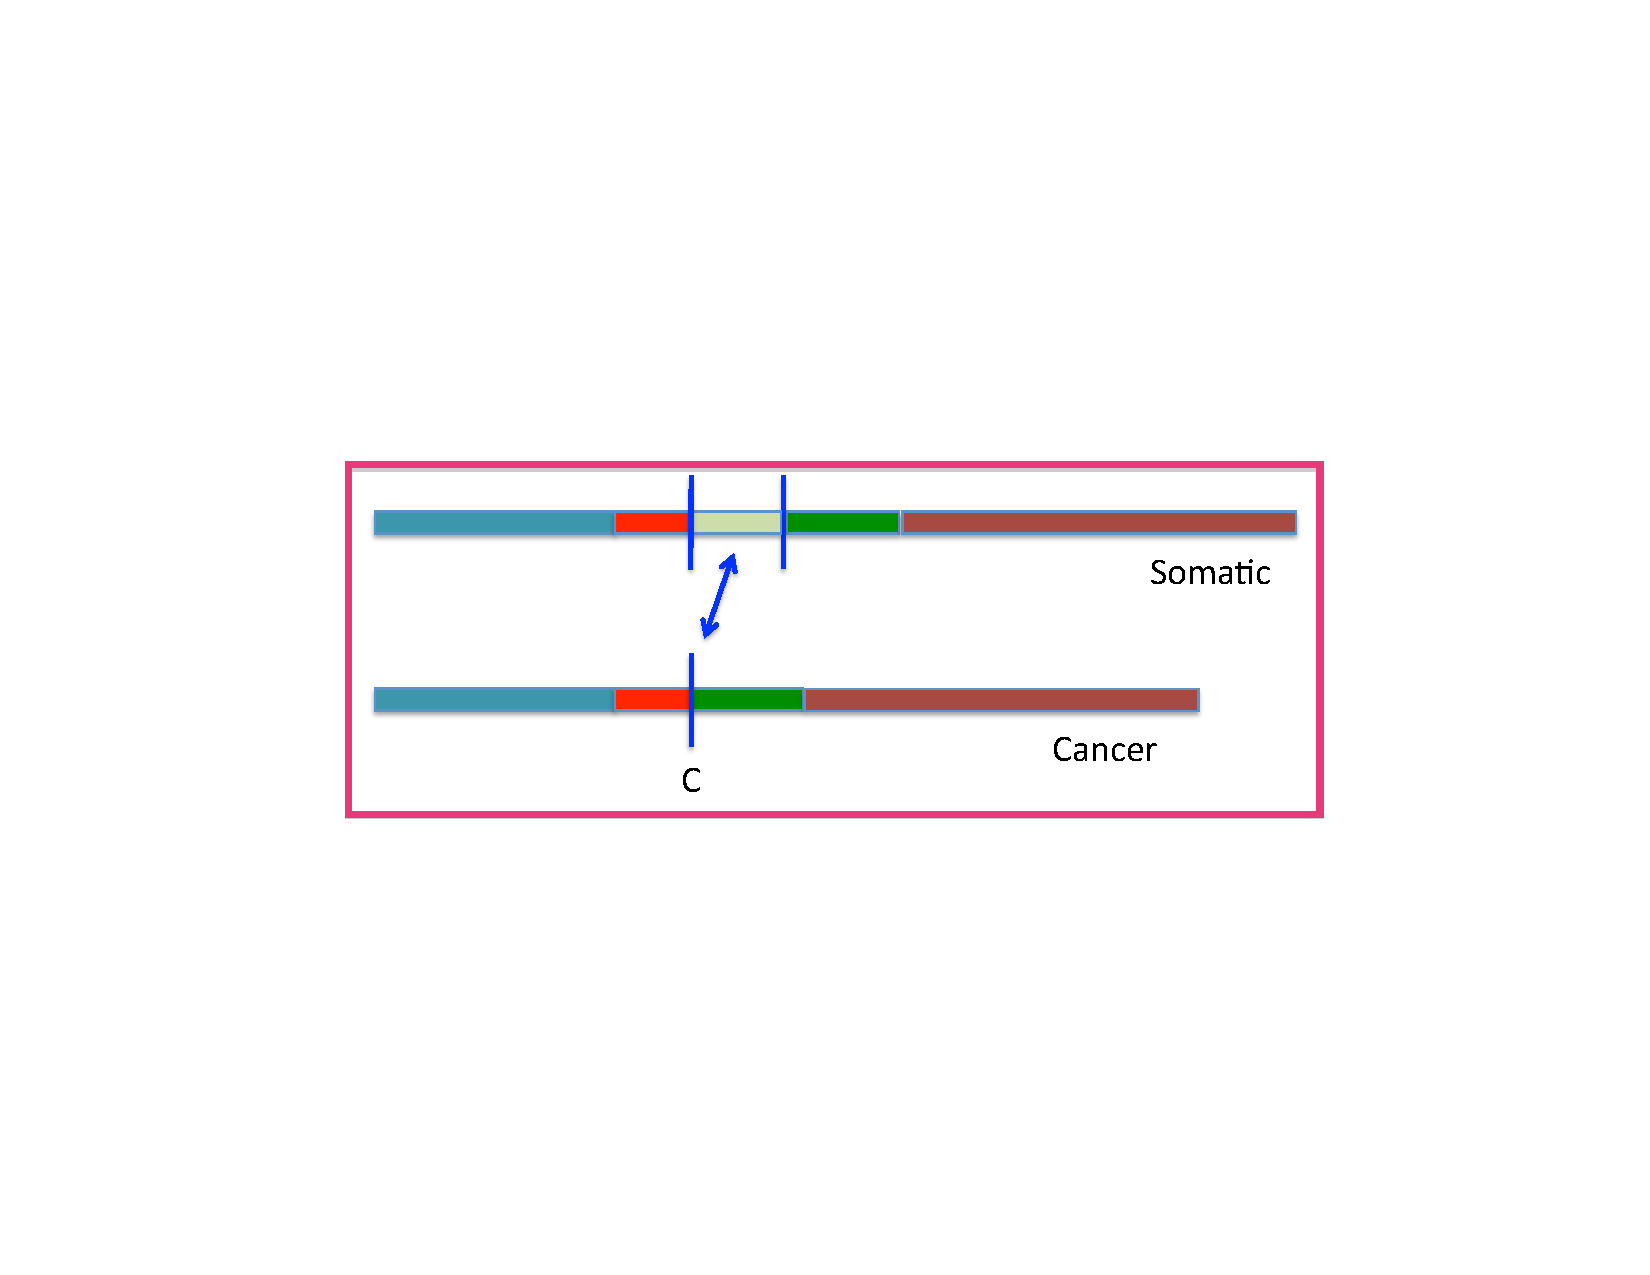
\includegraphics[width = 0.95  \linewidth]{../Code/Figures/DeletionDirect.pdf}
	\label{fig:DeletionDirect}}
%
\caption{{\bf Indirect vs direct comparison of deletion nested in insertion.} In the indirect comparison, the entire inner region, whether with or without an additional somatic deletion, is novel and thus only its outer breakpoints are detected. These outer breakpoints, however, are not somatic mutations and are present in both the somatic and tumor genomes. Thus the inner breakpoint is overlooked. The direct comparison, in contrast, ignores the outer breakpoints, as they are not different from the somatic to cancer genomes (only differ between genomes and reference). It instead only directs the somatic breakpoints, as these differ between the somatic and cancer genomes.}
\label{fig:NestedDeletion}
\end{figure}

\chapter{Materials and Methods}

\section{SV Detection Method}
\subsection{Initial Step-Wise Assemblies}
Because the somatic and cancer genomes are being compared directly to one another, the first step in this method is to assemble each genome. Reference-guided assembly is almost essential for a usable assembly of a genome as complex as the human genome. First the somatic genome is assembled using the human genome GRCh37 as a reference. Next, the tumor reads are assembled using the now assembled somatic genome as a reference. Using the somatic genome as a reference for the tumor genome minimizes the possibility of having false differences between the genomes. If there is a mistake in the assembly of the somatic genome, for instance, then an independent correct assembly of the cancer genome would incorrectly detect an SV at this position. However, if the cancer genome is assembled using the somatic as a reference, this error would likely be propagated to the cancer genome, and while not ideal to have an incorrect assembly, an incorrect breakpoint would not be called. Another reason for this choice is that the tumor genome is actually derived from the somatic, so there should be a very high degree of similarity between the two.

\begin{figure}[!ht]
\begin{center}
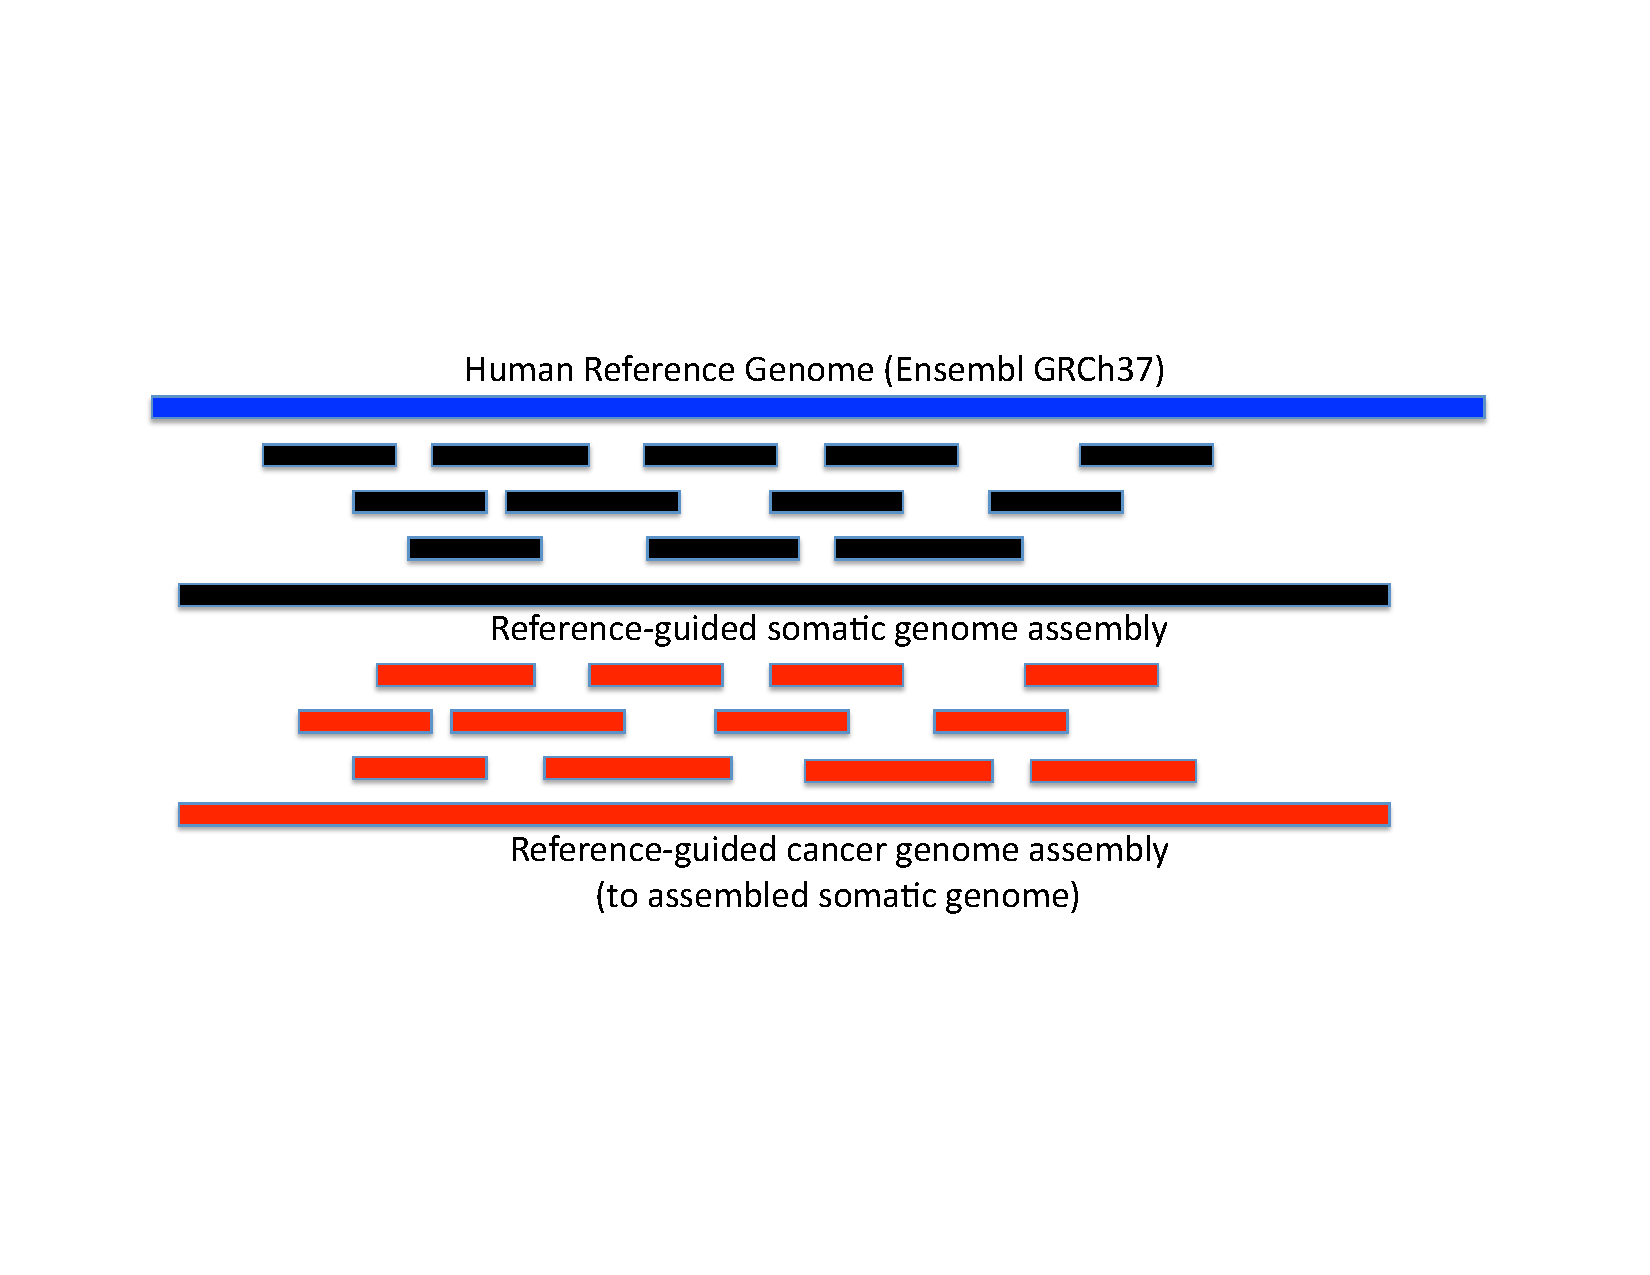
\includegraphics[width = 0.95  \linewidth]{../Code/Figures/RefGuidedAssembly.pdf}
\end{center}
\caption{{\bf Reference-guided assembly.}  The reads from the somatic genome are assembled using the human reference genome GRCh37 as a reference. Then the tumor reads are in turn assembled using the now assembled somatic genome as a reference.}
\label{fig:RefGuidedAssembly}
\end{figure}

\subsection{Alignments}
These reference sequences are first indexed with bowtie2 \cite{langmead2012fast} using the default parameters. This allows for easy referencing once the opposing reads are mapped onto each genome. We then map the raw tumor reads to the assembled somatic genome and the somatic reads to the assembled tumor genome using bowtie2. The cross-mapping is an essential step for two reasons. First, soft-clipped read SV detection has a bias towards detecting deletions rather than insertions. This is because when we map a read from a deletion, each side of the read should partially map to a region flanking the deleted region on the reference sequence. When both sides partially map, we can call this event with higher confidence. In a novel insertion, however, only the non-novel region can map to the reference, reducing confidence in half and greatly reducing our discovery rate. When we map in both directions, we should ideally detect both the insertion event on one genome and the deletion on the other. This provides us with two possible situations: either only one event, the insertion or more likely the deletion, is detected. In this case, we either have a false positive or false negative, as where there is an indel in one genome there must also be the oppoiste in the other genome. Because insertions are difficult to detect, we may indeed pick up some novel indel events as singular deletion events in one genome that would otherwise be missed checking for an insertion in one direction. Our first output is these singular events as a list of potential SVs that may be missed with traditional methods that only map reads in one direction, and expect to recover some number of novel insertion events missed by the deletion bias.

\begin{figure}[!ht]
\begin{center}
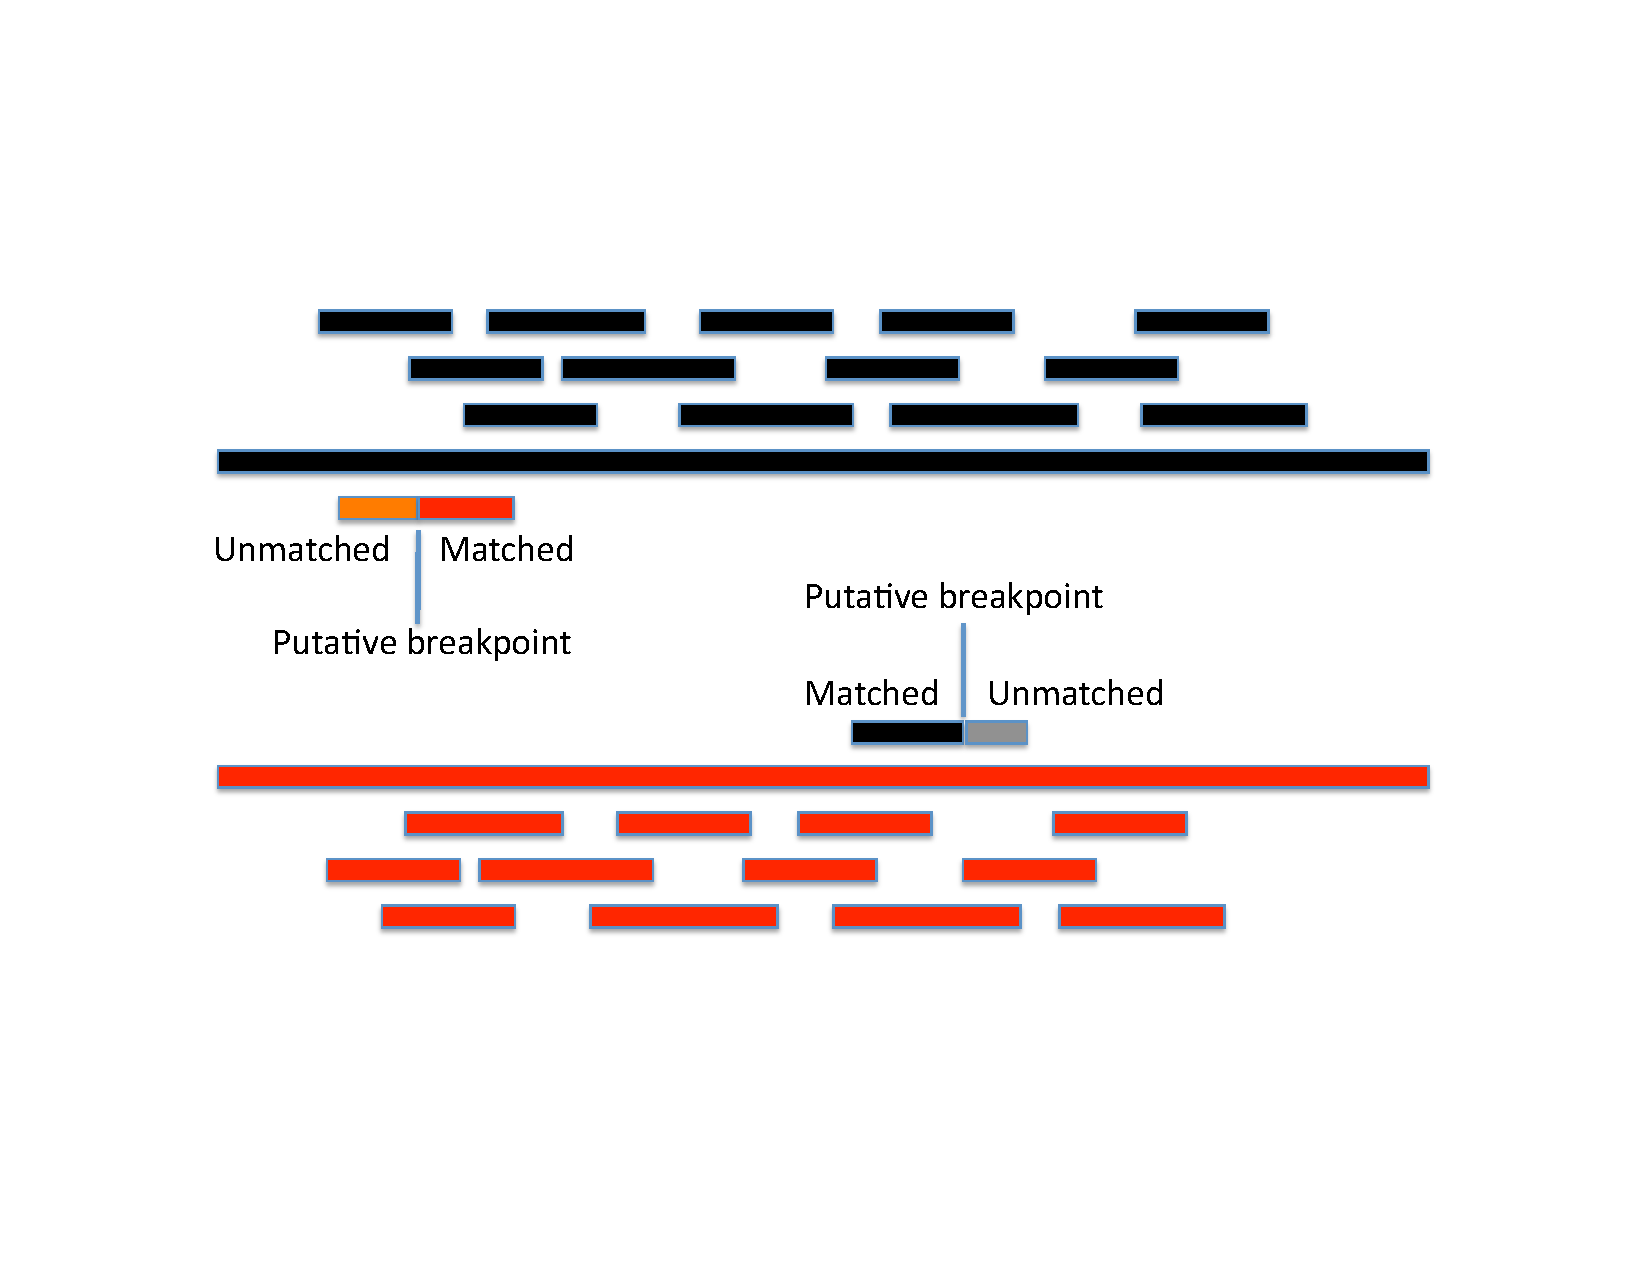
\includegraphics[width = 0.95  \linewidth]{../Code/Figures/SplitReadMapping.pdf}
\end{center}
\caption{{\bf Split-read mapping.}  When a read only partially maps to the opposing genome, the position at which there is no longer a match provides a putitive breakpoint for an SV in this position. We map somatic reads to the tumor genome and tumor reads to the somatic genome and compare split reads from both, as all true SVs should be detected on both genomes.}
\label{fig:SplitReadMapping}
\end{figure}

Our second output is a list of events that are detected in both genomes, which gives us higher confidence that they are true events. This is especially helpful for split-read detection, as it generally has a high false positive rate for breakpoint calling \cite{abel2013detection}. Having a list of high confidence breakpoints is a very helpful tool when wanting to extend the analyses further. Confirming breakpoints with Sanger sequencing is a common technique, but due to the high monetary and temporal cost of local sequencing, a small subset of the breakpoints is generally used \cite{jiang2012prism}. Thus only the most promising breakpoints should be chosen. This output would provide a solid initial subset for further sequencing and analyses.

Pindel and PRISM only perform with 26.3-37.6\% recall on real data for indels 21-100bp in length \cite{jiang2012prism}, demonstrating the need for higher accuracy provided with the first, single-hit output. Further, both of these methods had extremely low precision, $<$4\%, on indels 51-100 bp \cite{jiang2012prism}, showing a great need for a refined list of breakpoints, which is provided in the second, dual-hit output.

\subsection{SV Calling}
Samtools is used to convert the bowtie2 SAM output file into BAM format. The somatic and cancer alignment files are then each used as an input for Socrates to call breakpoints. [EXPLAIN WORKFLOW OF SOCRATES.]

From the Socrates output of breakpoints, a custom java program extracts and outputs the sequences flanking either side of each breakpoint into a FASTA file. These are then prepared for cross-checking for matches on each genome by indexing each FASTA file with bowtie2. To check for matching events between genomes, each FASTA file of flanking regions is mapped to the opposing indexed FASTA file using bowtie2 (we check both directions in case of a length difference, in which case the shorter may be mapped to the longer but not vice versa).

We then use another java program to determine which breakpoints correspond. There is a correspondence if 1) flanking regions from a given breakpoint in the cancer genome map to a breakpoint in the somatic genome and 2) flanking regions from that same breakpoint in the somatic genome map back onto the breakpoint in the cancer genome.

This system of comparing flanking regions to identify correpsonding breakpoints is based upon the characteristic that every breakpoint should have at least one flanking side conserved between the original and derived genomes.

\begin{figure}[!ht]
\begin{center}
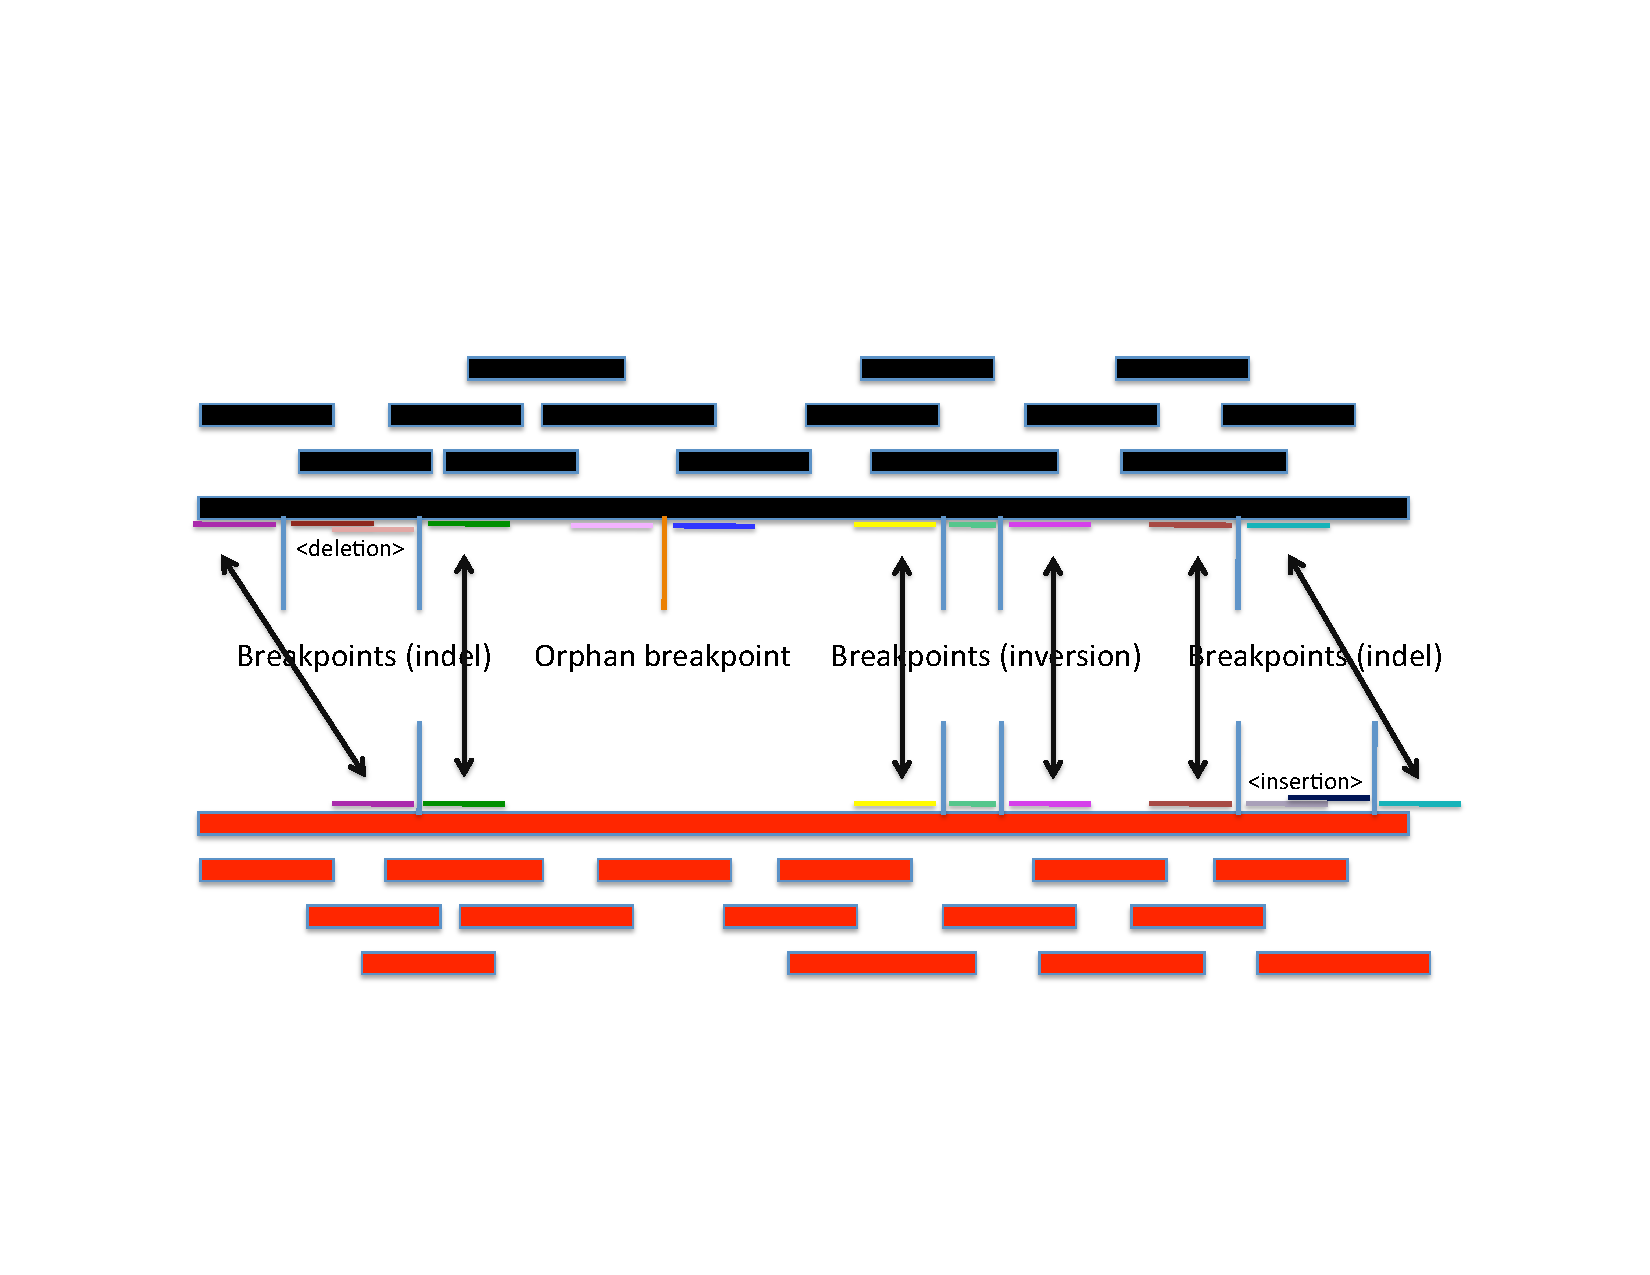
\includegraphics[width = 0.95  \linewidth]{../Code/Figures/FlankConservation.pdf}
\end{center}
\caption{{\bf Conservation of sequences flanking breakpoints.} In any type of SV, the region just beyond the breakpoint is unaffected and thus conserved between the original and derived genomes. Note that the orphan breakpoint would be on the first output list (detected in one direction), while those that map to a corresponding breakpoint would be on the second output list (detected in both directions).}
\label{fig:FlankConservation}
\end{figure}

\subsection{SV Annotation}
[Regions near the detected breakpoints will be run on ANNOVAR using the stored location on the reference genome to determine if it is a previously discovered SV. If there is no annotation, the region will be blasted, and the function of this region will be inferred for some number of breakpoints. The results from the low confidence (one direction mapped) and high confidence (both directions mapped) outputs will be compared.]

\section{Ideal Assembly}

\subsection{Simulate SVs}
I wrote a script in \texttt{Python 3} to simulate SVs in a chromosome. The inputs are the file name of the original sequence; the name of the sequence to be output; and the number of events to be simulated, which we call $N$. To generate the location of the start of the first SV event, the length of the chromosome is divided by $N$ and a location between 0 and $L/N$ is chosen. An event type is then chosen, all equally probable, with possibilities being a novel insertion, deletion, inversion, or translocation. The randomly selected event then occurs at the chosen position. $L$ is then updated after the first event, and the start location of the second event is then chosen randomly between $L/N$ and $2*(L/N)$. An event type is again randomly chosen, occurs at the start location, $L$ is updated, and the next event occurs between the next segment of length $L/N$. This occurs N number of times.

Insertions were simulated by drawing a random integer for its length, $L$, between 1 and 10,000. Then a sequence is generated by selecting a base, chosen randomly from "G", "C", "A", or "T", $L$ number of times and concatenating these into the novel insert. 

Deletions and inversion were simulated similarly, with a region of length $L$ between 1 and 10,000 to be removed and inverted, respectively.

When a translocation was called, the initial region is subject to the deletion. Then a location is chosen randomly throughout the entire genome for the region to be reinserted.

The outputs are the simulated genome, along with a list of breakpoints on this simulated genome and a list of corresponding breakpoints on the original reference sequence.

This script was then run on GRCh37 chromosome 11 with the number of events set to 20 to generate our "somatic genome," a simulated population variant from the reference. The script was then run again on this simulated chromosome with the number of events also set to 20 to generate a "cancer genome" derived from the somatic genome.

\subsection{Ideal Analysis}
I investigated how the direct comparison method compares to others (and of most direct interest, Socrates, which it is derived from) under the most ideal, error-free conditions, as a proof of concept and to reveal the maximum potential of the method. To perform this analysis, data was generated with no errors in the reads and a correct assembly given. The "somatic" reference genome was generated from running the SV simulation script on the GRCh37 human chromosome 11. The "cancer" reference genome was then built from running the same script on the "somatic" genome. Then from these two reference genomes, reads were generated with 0\% error from the DWGSIM software. The direct comparison pipeline was then run on the resulting reads and reference genomes with varying degrees of "known information." The first simulation assumes that the true genome assemblies are known, serving as a proof of concept under the best possible circumstances. The second simulation is the analog of what a real run would provide, assuming we do not know the assemblies and must build these from only the raw reads and a reference. Both of these versions of the pipelione are then compared with standard implementation of other common breakpoint detectors, which only utilize raw reads and the reference genome.

\section{Real Data}
I will then apply the method (analogous to simulation 2) to a real set of cancer NGS data - a somatic/tumor pair from individuals with thyroid cancer, accessed from NCBI's Gene Expression Omnibus accession number GSE48850.

\chapter{Results}

[The tables are filled with "0" and "N" as place-holders until the real results are obtained.]

\section{Ideal Analysis Performance}
Two types of simulations were run with varying levels of ideal information available. Simulation 1 supposes we know the true assemblies of both the somatic and cancer genomes. Thus this is the most possible information we can have and represents the best possible performance of the direct comparison pipeline. Note that this information is only utilized in the direct comparison method, giving a large advantage to the direct comparison method when this information is known. Both of the genomes along with the reads are used as inputs for the direct comparison method, while the raw reads and reference genome are used as inputs to the other tools.

Simulation 2 supposes we only have the raw reads available, which is the information we should have for a real run. Thus for the direct comparison method, the somatic genome is built through reference-guided assembly of the somatic reads to GRCh37 with default parameters in SHEAR \cite{landman2014shear}, as would be necessary in most applications. The tumor genome is then assembled through reference-guided assembly of the tumor reads to the just-built somatic genome. These two assembled genomes and the raw reads are given as inputs to the direct comparison method.

A final simulation only was performed to test for the detection of SVs nested within regions unique to the somatic genome (population-level variation). Thus only insertions were simulated when generating the somatic genome from the GRCh37 reference, and then further SVs in the cancer genome were only generated within these novel regions. Theoretically, the standard implementation of the tools (indirect comparison) should not detect any of these somatic mutations, while the direct comparison should be able to detect them with ease.

[Discuss comparison of direct comparison pipeline performance ideally and without known assemblies to the performance of running Socrates and the other tools with their standard implementations.]

\begin{table}[h]
\begin{center}
\begin{tabular}{|c|c|c|c|c|c|}\hline
         & Deletion & Insertion & Inversion & Transloc. Ins. & Transloc. Del.\\
        \hline 
        Ideal DC HR & 0 & 0 & 0 & 0 & 0\\
        Ideal DC FP & 0 & 0 & 0 & 0 & 0\\
        \hline 
        Assembled DC HR & 0 & 0 & 0 & 0 & 0\\
        Assembled DC FP & 0 & 0 & 0 & 0 & 0\\
        \hline
        Socrates HR & 0 & 0 & 0 & 0 & 0\\
        Socrates FP & 0 & 0 & 0 & 0 & 0\\
        \hline
        SHEAR HR & 0 & 0 & 0 & 0 & 0\\
        SHEAR FP & 0 & 0 & 0 & 0 & 0\\
        \hline
        PRISM HR & 0 & 0 & 0 & 0 & 0\\
        PRISM FP & 0 & 0 & 0 & 0 & 0\\
	\hline
\end{tabular}
\caption{{\bf Performance comparisons on simulated data set across all tools.} Data is averaged across 100 simulations. "Ideal DC" represents the direct comparison method when the ideal assemblies were supposed as known. "Assembled DC" represents the direct comparison method when the genomes were built from the raw reads. A hit represents correct identification/classification of an SV, and $HR = \# Hits / (\# Hits + \# False Negatives)$. A false positive is a called SV that did not actually occur, and $FP = \# False Positives / (\# False Positives + \# True Negatives)$.}
\end{center}
\end{table}

\begin{table}[h]
\begin{center}
\begin{tabular}{|c|c|c|c|}\hline
         & Nested Deletion & Nested Insertion & Nested Inversion\\
        \hline 
        Ideal DC HR & 0 & 0 & 0\\
        Ideal DC FP & 0 & 0 & 0\\
        \hline 
        Assembled DC HR & 0 & 0 & 0\\
        Assembled DC FP & 0 & 0 & 0\\
        \hline
        Socrates HR & 0 & 0 & 0\\
        Socrates FP & 0 & 0 & 0\\
        \hline
        SHEAR HR & 0 & 0 & 0\\
        SHEAR FP & 0 & 0 & 0\\
        \hline
        PRISM HR & 0 & 0 & 0\\
        PRISM FP & 0 & 0 & 0\\
	\hline
\end{tabular}
\caption{{\bf Performance comparisons on simulated data set with nested SVs.} Data is averaged across 100 simulations. All somatic mutations occured within a novel somatic region. In theory, all non-DC methods should miss these events and make no somatic mutation predictions. The DC method should be able to detect these events, but may be confounded by incorrect assembly, explaining the degredation in scores for the "Assembled DC" from the "Ideal DC."}
\end{center}
\end{table}


\section{Real Data Performance}
\subsection{Comparison to Socrates}

The ability to detect actual recorded mutations was then tested. Raw reads and a list of identified SVs from pediatric thyroid cancer cases near Chernobyl were used for this testing \cite{ricarte2013identification}. Predicted SVs with methods other than the DC pipeline could be compared to these mutations directly using Hg19 as a reference, as they both then identify SVs based upon the location on this same reference. A drawback of the DC pipeline with today's infrastructure is that because SV locations are given as positions on personalized genomes, an absolute position to a reference cannot be used for comparison. Instead, a sequence-based approach must be used, and thus the region where an SV was detected in the DC pipeline was subsequently manually blasted in NCBI's RefSeq, and the corresponding location/gene information was compared to that of the known SVs.

\begin{table}[h]
\begin{center}
\hspace*{-2.9cm}
\begin{tabular}{|c|c|c|c|c|c|}\hline
        \bf{Gene 1} & \bf{Chromosome 1/Position 1} & \bf{DC} & \bf{Socrates} & \bf{SHEAR} & \bf{PRISM}\\
        \hline 
        NBPF9 & 1, 144680292 & N & N & N & N\\
        \hline
        SLC2A5 & 1, 9121960 & N & N & N & N\\
        \hline
        RET & 10, 43611594 & N & N & N & N\\
        \hline
        DDX10 & 11, 108586716 & N & N & N & N\\
        \hline
        ENOX1 & 13, 44069703 & N & N & N & N\\
        \hline
        TYRO3 & 15, 41853839 & N & N & N & N\\
        \hline
        NAA60 & 16, 3528177  & N & N & N & N\\
        \hline
        WWP2 & 16, 69932549  & N & N & N & N\\
        \hline
        ERBB4 & 2, 212279972  & N & N & N & N\\
        \hline
        MTA3 & 2, 42798222  & N & N & N & N\\
        \hline
        DPP10 & 2, 116377141  & N & N & N & N\\
        \hline
        BAGE3,BAGE2,BAGE5,BAGE4 & 21, 11023095 & N & N & N & N\\
        \hline
        CRTAP & 3, 33176800 & N & N & N & N\\
        \hline
        FAM13A & 4, 89672634 & N & N & N & N\\
        \hline
        PHACTR1 & 6, 13191467 & N & N & N & N\\
        \hline
        CBX3 & 7, 26252774 & N & N & N & N\\
        \hline
        STAG3L4 & 7, 66769841 & N & N & N & N\\
        \hline
        LOC642236 & 9, 68434485  & N & N & N & N\\
        \hline
\end{tabular}
\caption{{\bf Detection of somatic chromosomal rearrangements in thyroid somatic/cancer pair.} Somatic/cancer raw reads are taken from sample T1\cite{ricarte2013identification}, and Hg19 is used as the reference. "N" corresponds to this SV not being called, while "Y" corresponds to this SV being called. All SVs should be true and thus called with a "Y."}
\hspace*{-2.9cm}
\end{center}
\end{table}

\subsection{Novel Predictions}
[Likely novel results that appeared in the direct comparison method that were not present in the existing SV set or Socrates output. Will also determined if there is an improvement in the deletion bias with the DC method.]

\begin{table}[h]
\begin{center}
\begin{tabular}{|c|c|c|}\hline
         & \# Deletions Called & \# Insertions Called\\
        \hline 
        DC Out 1 & 0 & 0\\
        DC Out 2 & 0 & 0\\
        \hline 
        Socrates & 0 & 0\\
        \hline
        SHEAR & 0 & 0\\
        \hline
        PRISM HR & 0 & 0\\
	\hline
\end{tabular}
\caption{{\bf Insertions/deletions called in thyroid somatic/cancer pair.} "DC Out 1" represents those indels called in the first output of the direct comparison method, which is the high-confidence dual-mapped list. "DC Out 1" represents those indels called in the second output of the direct comparison method, which is the lower-confidence single-mapped list.}
\end{center}
\end{table}

\chapter{Discussion}
\section{Applications of this pipeline}
[Will discuss the succusses and failures of each of the two outputs in the simulations:
	1) Did the first output provide us with additional, true breakpoints?\\
	2) Did the second output have a higher hit rate and lower false positive rate?\\
Was there less of a bias towards deletions in the DC method with the number of predicted indels?]

[Results pending: The simulations show the lack of ability for standard methods to detect any SVs within a novel region, which in some sense we couldn't have known what we are missing. The concept of direct comparison has the potential to resolve this issue, as we see most of these events are called when comparing directly. We expect these events to be fairly common, as there is much population level variation among humans, and rare variants are increasingly being found to play a role in genetic disease prevalence.

We also see from the ideal results that there is a deletion bias in the traditional methods and also that bidirectional mapping has the potential to drastically reduce this bias. However, the limiting step in this method in particular is the reliance upon an initial assembly, which reduced the accuracy of all SV calls.]

This method is not desigend to replace other methods for detecting SVs, but primarily to fill in the gap of novel insertions and nested SVs that would likely otherwise go unnoticed. Thus this method would be best used in supplement with methods that do not rely on assemblies and can find majority of the easier-detected deletions, smaller indels, SNPs, etc.

\section{Future directions}
This pipeline can be used with any reference-guided assembler and breakpoint detector, so it will improve with advances in these tools. As assembly is a huge limiting step in this pipeline, the next step would be to modify the pipeline to compare reads directly rather than first making draft assemblies. Another option would be to adapt the assembly in progress by using the predicted breakpoints. SHEAR \cite{landman2014shear} uses such a back-and-forth breakpoint predictor/assembler, but this specific tool still compares reads indirectly to the reference.

As other methods shift towards providing a full, personalized genome, the standard for SV annotation should shift from being anchored to location on a reference to relying solely on sequence look-up. It is almost counter-intuitive to reference 2 different locations in 2 genomes by a third different location in the reference sequence when all 3 share common sequence, and this is actually inhibitory when technology allows us to move further away from reliance on a single reference genome. Both a shift towards sequence-lookup or the above suggested change to direct read comparison would help resolve the issue encountered with this specific method of manual annotation.

Though the technology may not yet be at a place where this implementation of the method is more advantageous than the standard indirect comparison SV detectors, the largely overlooked limitations of indirect comparison, namely deletion bias and failure to detect nested SVs, are brought to light here; further, a general method, direct bi-directional mapping, is offered to overcome both of these. While the traditional methods encounter these issues at a fundamental level and will remain stagnant to them regardless of technological advances, this method should improve with both sequencing and assembling technology, offering a potential avenue for future SV detection.

%
% Appendices
%
%\appendix
%\chapter{Incomplete Discography I}.
%Here's a table of some Yes Albums I can think of, in something that's 
%close to but certainly not in chronological order.

%\chapter{Useless figures}
%Here's a pointless figure:
%\begin{figure}[htbp]
%  \begin{center}
%    {\Huge Yes!}
%    \caption{Yes}
%  \end{center}
%\end{figure}
%and another:
%\begin{figure}[htbp]
%   \begin{center}
%     {\Huge No!}
%     \caption{No}
%    \end{center}
%\end{figure}

%
% References (the thesis office prefers that to Bibliography...)
%
% They also prefer that it be single spaced.
% The pagebreak command is necessary inorder to insure that 
%  the page number that appears in the table of contents is
%  the correct one.   

\singlespacing
\pagebreak
\addcontentsline{toc}{chapter}{References}

\bibliographystyle{ieeetr}
\nocite{*}
\bibliography{BibThesis}

%\begin{thebibliography}{99}
   % the 99 is as wide or wider than any bibliography labels.
%\bibitem{fragile}Anderson, Bruford, Squire, Wakeman.  \emph{Fragile}.
%  Atlantic, 1973.
%\end{thebibliography}

\end{document}